\chapter{Experiments and results}
\label{experiments_and_results}

The algorithm presented in this work was implemented and several experiments with a simple garment dataset were conducted. This chapter is devoted to explain the experiments performed using the algorithm presented in this thesis. It includes the implementation details, the experimental setup and the experiments themselves, as well as the results obtained through those experiments.

\section{Implementation details}
\label{experiments:implementation}
The software implementation for this thesis has two main parts. The first one is in charge of communication with the sensor with the objective of extracting the depth data. This communication is performed using YARP \cite{metta2006yarp}. YARP is a set of libraries, protocols, and tools that leverages many common tasks required for a humanoid robot to work. Those tasks include actuator control and command, communications with the robot and between software parts, and accessing to data captured from different common sensors, such as depth sensors.

The second one is the implementation of the unfolding algorithm. This implementation was executed using Python\footnote{\url{http://www.python.org}} as our language of choice. Python is a programming language that allows a quick development of prototype software, and that counts with a large collection of external modules to perform several tasks, from math calculations to computer vision. Our implementation is based on tho different computer vision libraries: OpenCV\footnote{\url{http://www.opencv.org}} and Scikit-image\footnote{\url{http://scikit-image.org}}. We chose to use both since during the development of this work several algorithms were evaluated, and each library contains only a subset of those algorithms. In the latest version, OpenCV is used for basic computer vision and Scikit-image for more advanced algorithms such as Watershed \footnote{\url{http://scikit-image.org/docs/dev/auto_examples/plot_watershed.html}} and other superpixel-based clustering methods. 

The whole unfolding algorithm implementation is Open Source, and is available online\footnote{\url{https://github.com/roboticslab-uc3m/textiles}}.

\comment{Should I speak of the wonderful evaluation GUI tool?}

\section{Algorithm Evaluation}
\label{experiments:evaluation}

\comment{Bla, bla, bla... evaluation, bla, bla, bla}

\subsection{Garment Dataset}
\label{experiments:dataset}

To test the computer vision algorithm, a garment dataset was crafted\footnote{\url{http://tinyurl.com/garments-birdsEye-zip}}. Other garment datasets already existed, such as the ones provided by the CloPeMa project\footnote{\url{http://clopema.felk.cvut.cz/public_data.html}}, but they were not suitable to test our algorithm, since these datasets are mainly focused on modeling and folding garments once they are already extended. 

Our dataset is composed of 120 samples of different folds in garments from 6 different categories: skirt, jacket, pants, polo, robe and hoodie. Each category set is composed by 20 samples, 10 of which present one fold and 10 of which present two folds in the garment. This data was obtained using an ASUS Xtion PRO LIVE with RGB and depth channels set at 640x480 resolution. The sensor is placed on top of the working surface providing a bird's eye view over the garment folding environment, with its image plane almost parallel to the working surface.

\comment{Lorem ipsum dolor sit amet, consectetur adipiscing elit. Donec a diam lectus. Sed sit amet ipsum mauris. Maecenas congue ligula ac quam viverra nec consectetur ante hendrerit. Donec et mollis dolor. Praesent et diam eget libero egestas mattis sit amet vitae augue. Nam tincidunt congue enim, ut porta lorem lacinia consectetur. Donec ut libero sed arcu vehicula ultricies a non tortor. Lorem ipsum dolor sit amet, consectetur adipiscing elit. Aenean ut gravida lorem. Ut turpis felis, pulvinar a semper sed, adipiscing id dolor. Pellentesque auctor nisi id magna consequat sagittis. Curabitur dapibus enim sit amet elit pharetra tincidunt feugiat nisl imperdiet. Ut convallis libero in urna ultrices accumsan. Donec sed odio eros. Donec viverra mi quis quam pulvinar at malesuada arcu rhoncus. Cum sociis natoque penatibus et magnis dis parturient montes, nascetur ridiculus mus. In rutrum accumsan ultricies. Mauris vitae nisi at sem facilisis semper ac in est.}

\subsection{Experiments}
\label{experiments:experiments}

Fig. \ref{fig:results} shows the final output of the algorithm and the computed unfolding directions for 4 garments of each of the 6 categories.

For evaluating the algorithm, a scoring metric has been established. The criteria for the scoring is qualitative, due to the lack of an objective ground truth to provide quantitative comparisons. The output of each stage is manually classified into one of the following categories: \fail{}, \good{}, \great{} and \discarded{}. Results from one stage that prevent the next one to work properly are classified as \fail{}, and the next stages for that item are classified as \discarded{} and skipped. Results that are not perfect, but allow the next stage to compute its output are classified as \good{}. Note that the \good{} score in the last stage means that the robot could unfold it, but it is not the optimal path. Finally, perfect results for a stage are given the \great{} score. Table \ref{table:table} shows the raw data of this scoring, indicating the amount of samples that received each score at a given stage for each category.


\begin{table}[t]
\centering
\hspace*{-1.25em}
\begin{tabular}{|r|rrrr|rrrr|}
\hline
	& \multicolumn{4}{|c|}{Skirt} &\multicolumn{4}{|c|}{Jacket}  \\
\hline
   Stage   & \fail & \good & \great & \discarded & \fail & \good & \great & \discarded \\
\hline
   Segmentation         &  0 & 0 & 20 &  0 &    0 & 9 & 11 &  0 \\
   Clustering           &  3 & 6 & 11 &  0 &    8 & 8 &  4 &  0 \\
   Pick \& Place        &  5 & 5 &  7 &  3 &    3 & 3 &  6 &  8 \\
\hline
\end{tabular}

\vspace{1em}
\hspace*{-1.25em}
\begin{tabular}{|r|rrrr|rrrr|}
\hline
	&\multicolumn{4}{|c|}{Pants} & \multicolumn{4}{|c|}{Polo}  \\
\hline
   Stage   &     \fail & \good & \great & \discarded & \fail & \good & \great & \discarded  \\
\hline
   Segmentation         &  1 & 1 & 18 &  0   & 0 & 17 &  3 &  0 \\
   Clustering           &  7 & 5 &  7 &  1   & 3 & 13 &  4 &  0 \\
   Pick \& Place        &  8 & 1 &  3 &  8   & 1 &  4 & 12 &  3 \\
\hline
\end{tabular}

\vspace{1em}
\hspace*{-1.25em}
\begin{tabular}{|r|rrrr|rrrr|}
\hline
	 &\multicolumn{4}{|c|}{Robe} &\multicolumn{4}{|c|}{Hoodie}   \\
\hline
   Stage   & \fail & \good & \great & \discarded & \fail & \good & \great & \discarded \\
\hline
   Segmentation         &   0 & 0 & 20 & 0 &   11 &  3 &  6 &  0\\
   Clustering           &   5 & 7 &  8 & 0 &    6 &  2 &  1 & 11\\
   Pick \& Place        &   3 & 3 &  8 & 6 &    3 &  0 &  0 & 17\\
\hline
\end{tabular}
\caption{Raw data results of the established scoring metric for each garment category and algorithm stage}
\label{table:table}
\end{table}


A stage by stage analysis is provided in Table \ref{table:table2}. Each cell represents the percent of \good{} and \great{} qualified samples with respect to the amount of samples that actually reached the given stage:

\begin{equation}
cell = \frac{\good + \great}{\fail + \good + \great} \cdot 100 \%
\end{equation}

The Overall performance included in the last row shows the percent of \good{} and \great{} samples taking into account all the samples, including the ones scored as \discarded{}, and corresponds to the product of the percentages of each individual stage, since they are independent events.

\begin{table}[t]
\centering
\begin{tabular}{|r||r|r|r|r|r|r||r|}
\hline
	Stage \slash{} Category & Skirt & Jacket & Pants & Polo & Robe & Hoodie & All \\
\hline\hline
   Segmentation         & 100   & 100 &  95   & 100   & 100   & 45   & \textbf{90}\\
   Clustering           &  85   &  60 &  63.2 &  85   &  75   & 33.3 & \textbf{70.4}\\
   Pick \& Place Points &  70.6 &  75 &  33.3 &  94.1 &  78.6 &  0   & \textbf{69.3}\\
   \hline\hline
   Overall              &  60   &  45 &  20   &  80   &    55 &  0   & \textbf{43.3} \\ 
\hline
\end{tabular}
\caption{Results analysis per stage and garment category, expressed in percentage (\%)}
\label{table:table2}
\end{table}

For instance, the Segmentation stage was evaluated as having performed correctly (which includes \good{} and \great{} samples) for 100\% of the Skirt category. With the remaining samples, the Clustering stage performance was evaluated. In this case, within the Skirt category, all of the Skirt samples were evaluated, because they had all passed the previous stage. In this evaluation, 85\% achieved a passing score (\good{} and \great{}). This set of samples was passed on to the Pick \& Place points stage, and for these samples, 70.6\% achieved a passing score within the Skirt category. The Overall algorithm performance for the category is computed as the product of the percentages of three stages: $1 \cdot 0.85 \cdot 0.70 = 60\%$ based on the 20 skirt samples. Table \ref{table:table2} includes an additional column which applies this process based on the evaluation of All the 120 samples of the dataset.

A final set of laboratory experiments to validate the unfolding algorithm have been performed using the full-size humanoid robot TEO \cite{martinez2012teo}. The robot's gripper, designed with passive compliance and relatively large objects in mind (e.g. fruit, bottles, etc), was substituted by a gripper for garment manipulation actuated with hobby servomotors. The garment data was obtained using the ASUS RGB-D sensor in the same configuration (at the ceiling) as for the dataset generation. 

Once the unfolding pick and place points are computed, depth sensor coordinates are converted to the robot root frame. A standard pick and place operation is performed with the final obtained points.



\begin{figure}[htbp]
	\centering
	%%%%%%%%%%%%%%%%%%%%%%%%%%%%%%%%%% FigA %%%%%%%%%%%%%%%%%%%%%%%%%%%%%%%%%%%%%%%%%%%%%
	\begin{subfigure}[l]{\bigtablewidth}
	    \centering
    	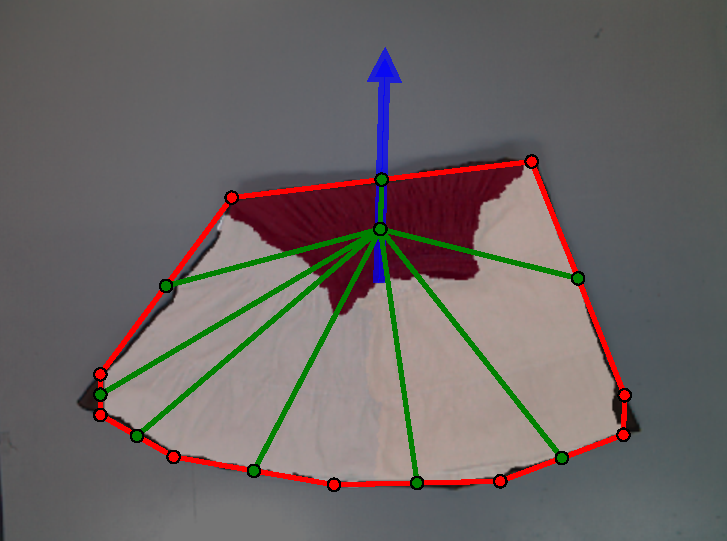
\includegraphics[width=\textwidth]
    	{figures/results/skirt3-pnp.pdf}
	\end{subfigure}
	~
	\begin{subfigure}[r]{\bigtablewidth}
	    \centering
    	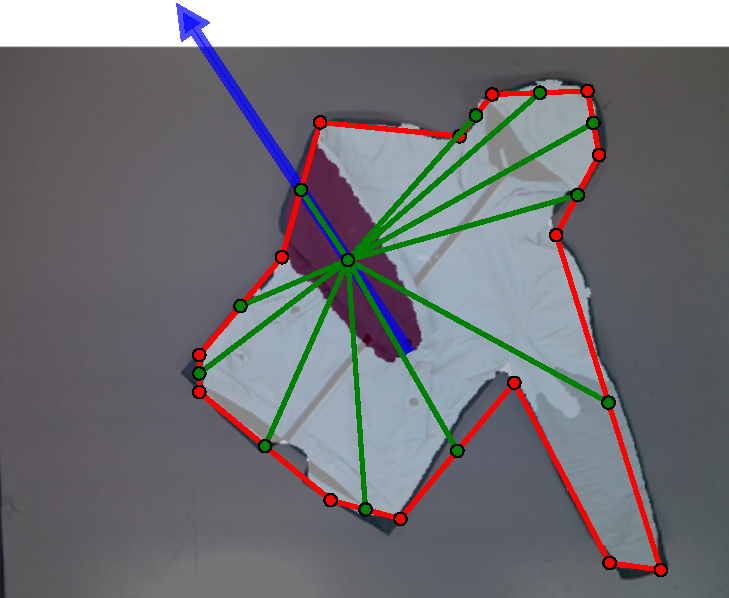
\includegraphics[width=\textwidth]
    	{figures/results/jacket1-pnp.pdf}
	\end{subfigure}
	~
    \begin{subfigure}[l]{\bigtablewidth}
	    \centering
    	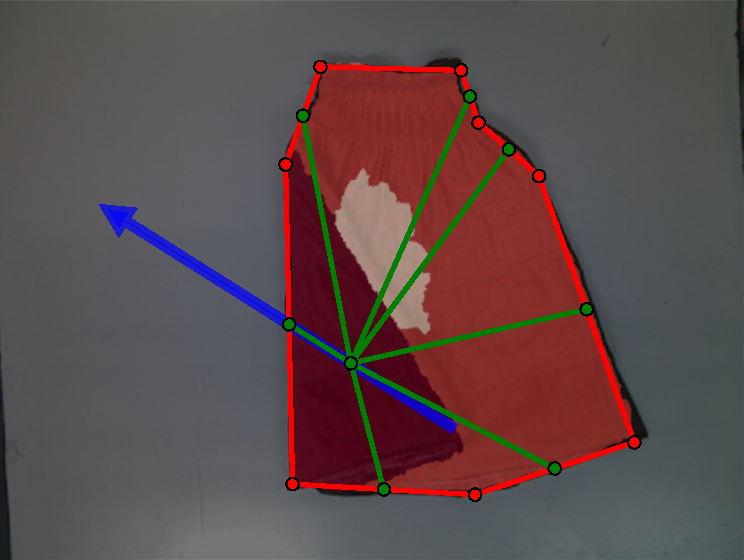
\includegraphics[width=\textwidth]
    	{figures/results/skirt7-pnp.pdf}
	\end{subfigure}
	~
    \begin{subfigure}[r]{\bigtablewidth}
	    \centering
    	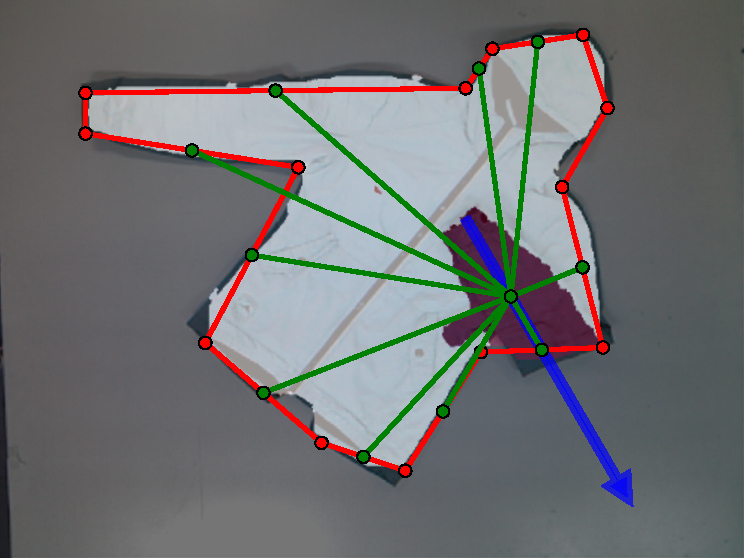
\includegraphics[width=\textwidth]
    	{figures/results/jacket2-pnp.pdf}
	\end{subfigure}
	~
    \begin{subfigure}[l]{\bigtablewidth}
	    \centering
    	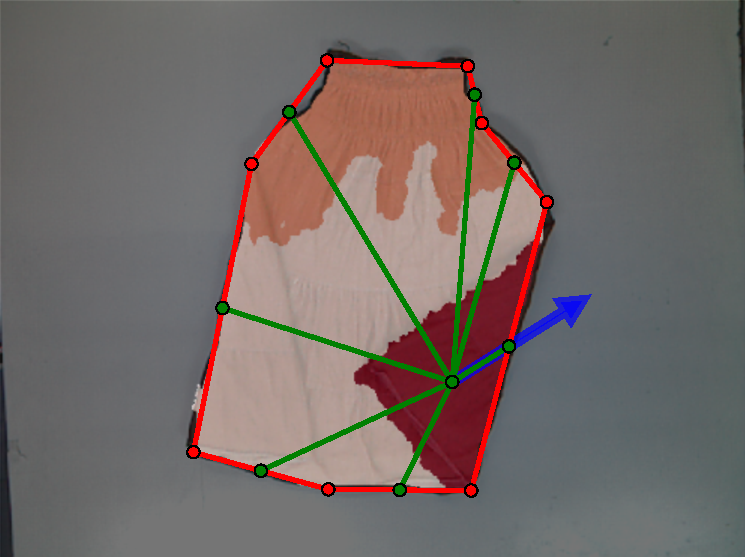
\includegraphics[width=\textwidth]
    	{figures/results/skirt13-pnp.pdf}
	\end{subfigure}
	~
    \begin{subfigure}[r]{\bigtablewidth}
	    \centering
    	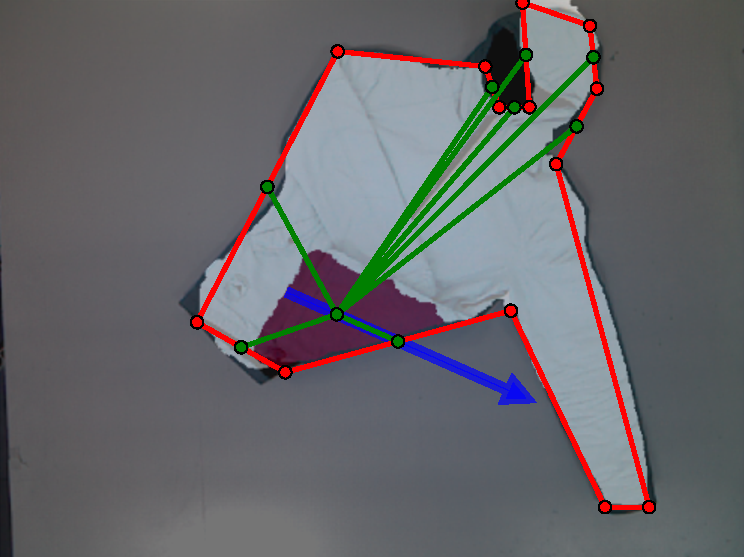
\includegraphics[width=\textwidth]
		{figures/results/jacket12-pnp.pdf}
	\end{subfigure}
	~
    \begin{subfigure}[l]{\bigtablewidth}
	    \centering
    	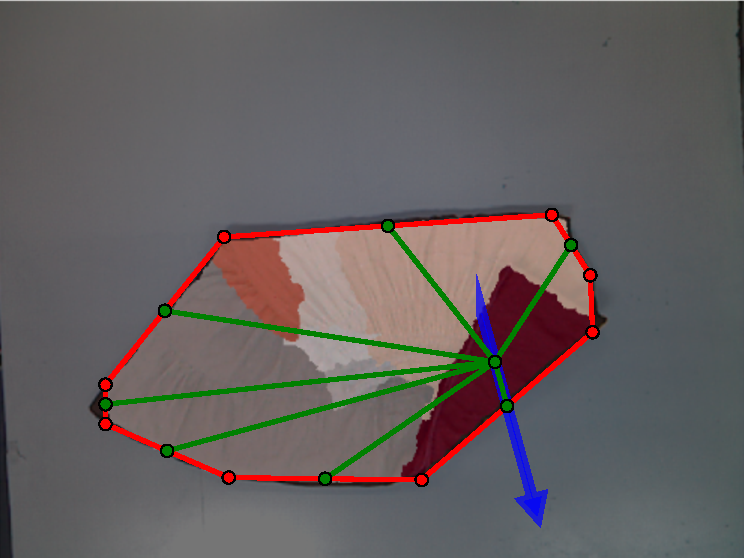
\includegraphics[width=\textwidth]
    	{figures/results/skirt19-pnp.pdf} 
	\end{subfigure}
	~
    \begin{subfigure}[r]{\bigtablewidth}
	    \centering
    	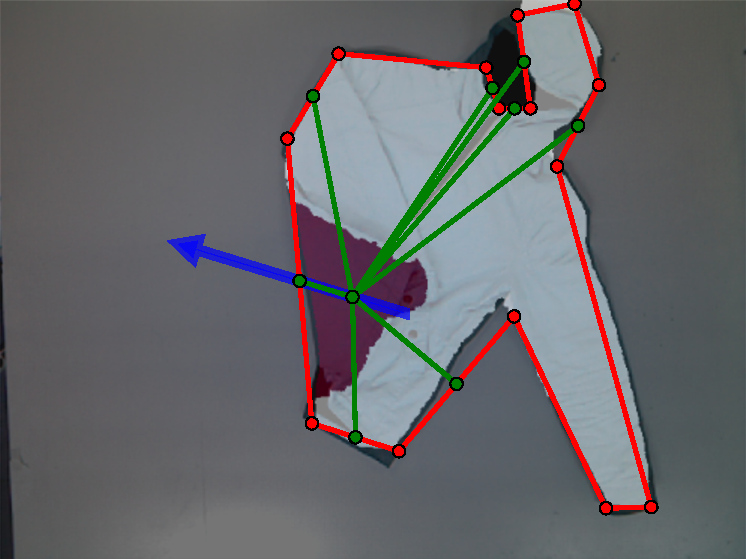
\includegraphics[width=\textwidth]
		{figures/results/jacket13-pnp.pdf}    	
	\end{subfigure}
    \caption[Final output of the algorithm and the computed unfolding directions (Skirt and jacket)]
    {Final output of the algorithm and the computed unfolding directions. Each column includes the output corresponding to 4 of the 20 database samples for each of the 6 garment categories considered. This figure includes the categories Skirt and Jacket.}
    \label{fig:results}
\end{figure}

\begin{figure}[htbp]
	\centering
	%%%%%%%%%%%%%%%%%%%%%%%%%%%%%%%%%% FigB %%%%%%%%%%%%%%%%%%%%%%%%%%%%%%%%%%%%%%%%%%%%%
	\begin{subfigure}[l]{\bigtablewidth}
	    \centering
    	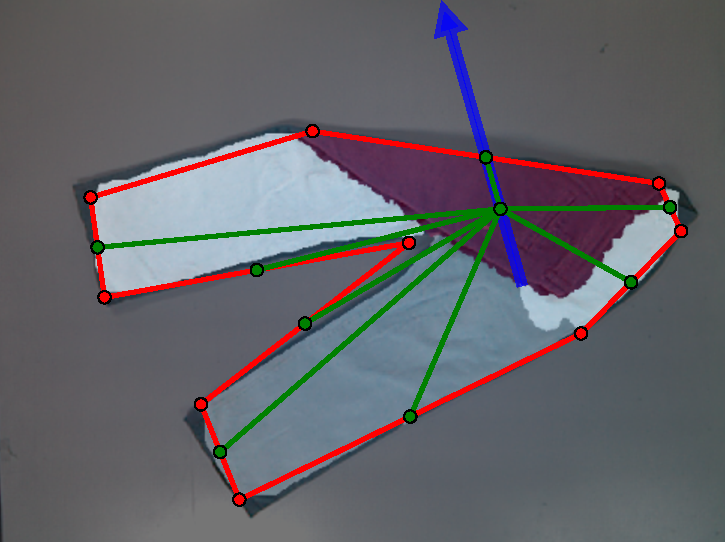
\includegraphics[width=\textwidth]
    	{figures/results/pants7-pnp.pdf}
	\end{subfigure}
	~
	\begin{subfigure}[r]{\bigtablewidth}
	    \centering
    	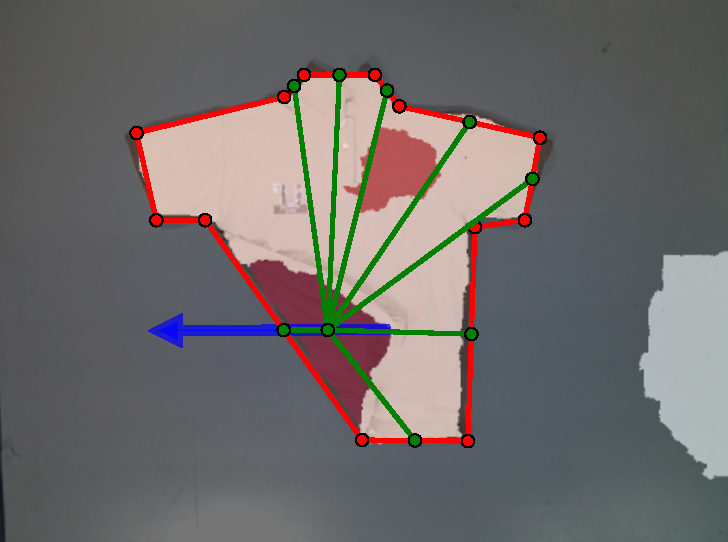
\includegraphics[width=\textwidth]
    	{figures/results/polo1-pnp.pdf}
	\end{subfigure}
	~
    \begin{subfigure}[l]{\bigtablewidth}
	    \centering
    	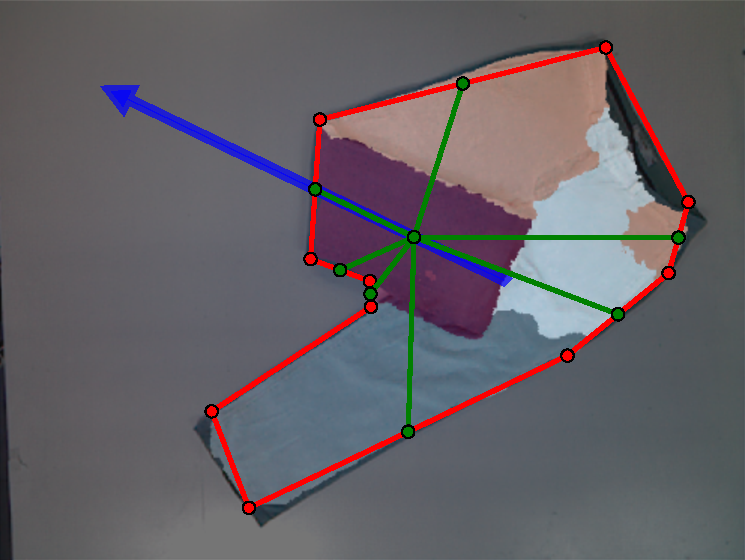
\includegraphics[width=\textwidth]
    	{figures/results/pants8-pnp.pdf}
	\end{subfigure}
	~
    \begin{subfigure}[r]{\bigtablewidth}
	    \centering
    	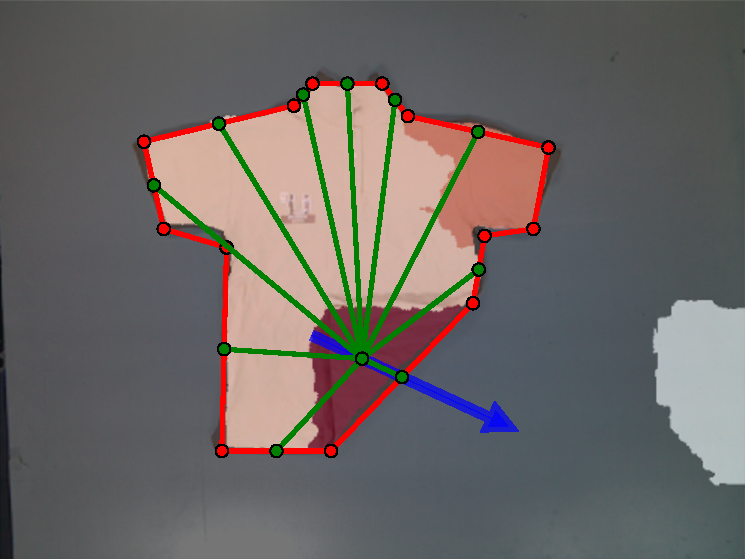
\includegraphics[width=\textwidth]
    	{figures/results/polo2-pnp.pdf}
	\end{subfigure}
	~
    \begin{subfigure}[l]{\bigtablewidth}
	    \centering
    	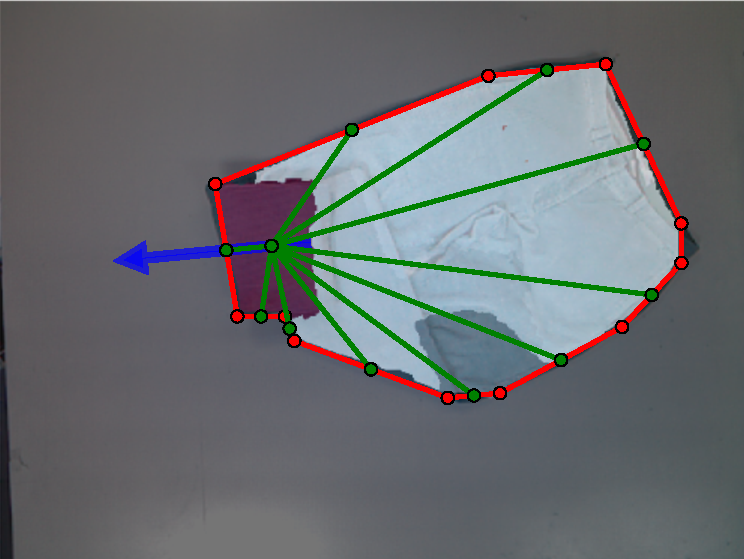
\includegraphics[width=\textwidth]
    	{figures/results/pants14-pnp.pdf}
	\end{subfigure}
	~
    \begin{subfigure}[r]{\bigtablewidth}
	    \centering
    	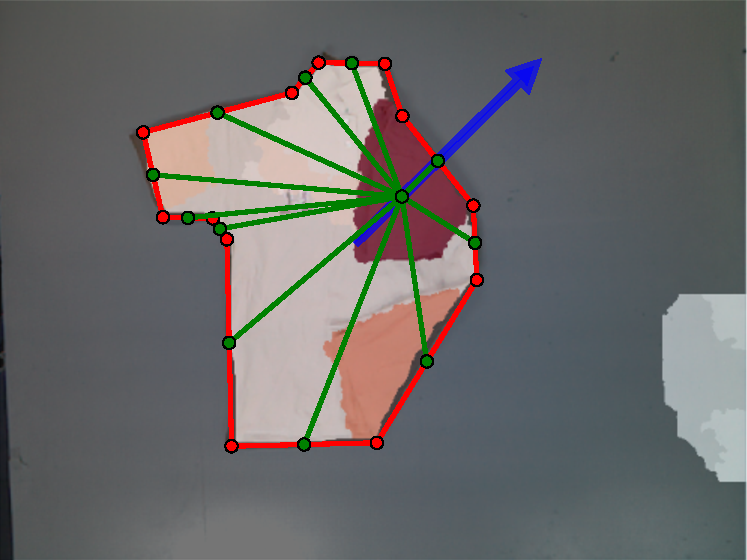
\includegraphics[width=\textwidth]
    	{figures/results/polo13-pnp.pdf}
	\end{subfigure}
	~
    \begin{subfigure}[l]{\bigtablewidth}
	    \centering
    	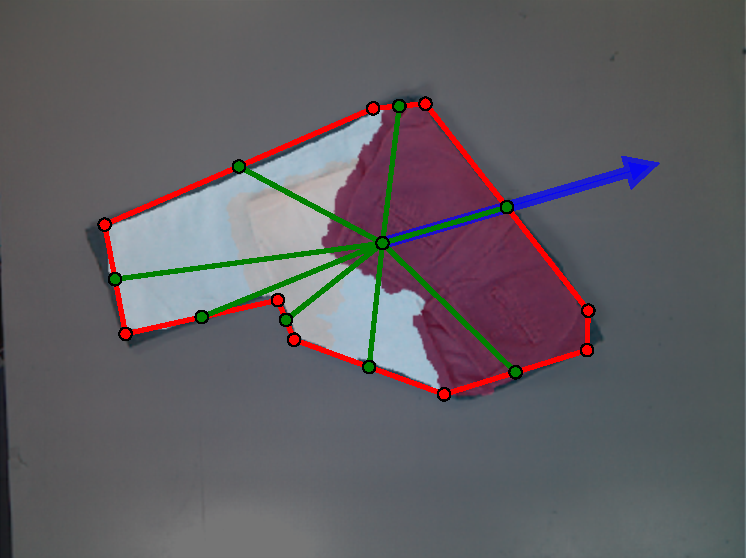
\includegraphics[width=\textwidth]
    	{figures/results/pants15-pnp.pdf}
	\end{subfigure}
	~
    \begin{subfigure}[r]{\bigtablewidth}
	    \centering
    	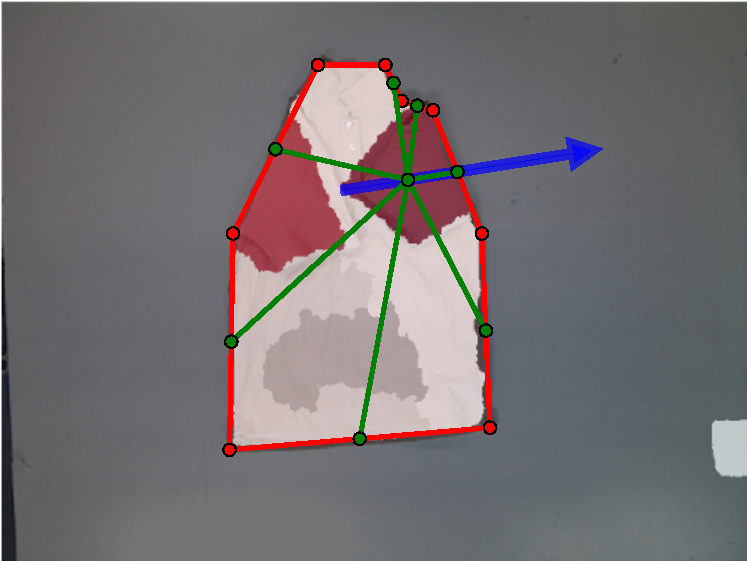
\includegraphics[width=\textwidth]
    	{figures/results/polo15-pnp.pdf}
	\end{subfigure}
	\caption[Final output of the algorithm and the computed unfolding directions (Pants and Polo).]
    {Final output of the algorithm and the computed unfolding directions. Each column includes the output corresponding to 4 of the 20 database samples for each of the 6 garment categories considered.This figure includes the categories Pants and Polo.}
    \label{fig:results2}
\end{figure}

\begin{figure}[htbp]
	\centering
	%%%%%%%%%%%%%%%%%%%%%%%%%%%%%%%%%% FigC %%%%%%%%%%%%%%%%%%%%%%%%%%%%%%%%%%%%%%%%%%%%%
	\begin{subfigure}[l]{\bigtablewidth}
	    \centering
    	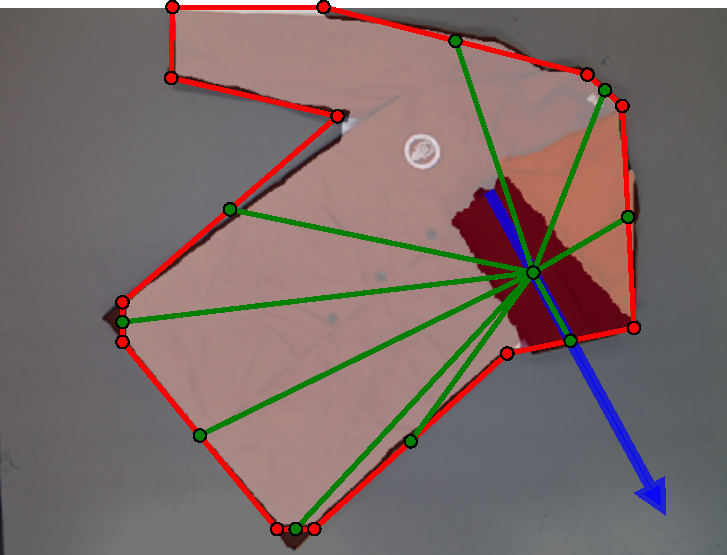
\includegraphics[width=\textwidth]
    	{figures/results/robe4-pnp.pdf}
	\end{subfigure}
	~
    \begin{subfigure}[r]{\bigtablewidth}
	    \centering
    	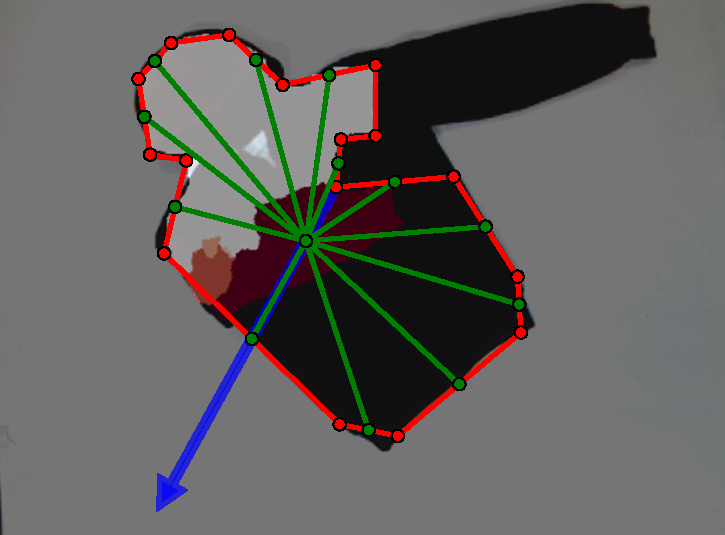
\includegraphics[width=\textwidth]
    	{figures/results/hoodie1-pnp.pdf}
	\end{subfigure}
	~
    \begin{subfigure}[l]{\bigtablewidth}
	    \centering
    	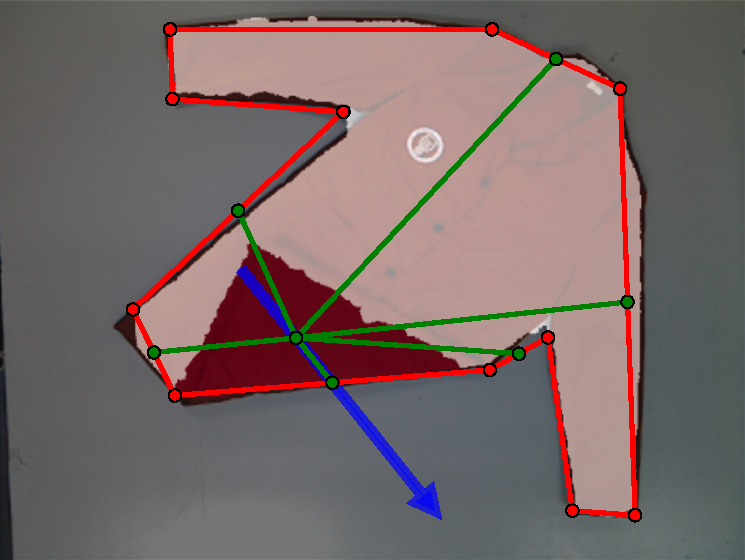
\includegraphics[width=\textwidth]
    	{figures/results/robe8-pnp.pdf}
	\end{subfigure}
	~
    \begin{subfigure}[r]{\bigtablewidth}
	    \centering
    	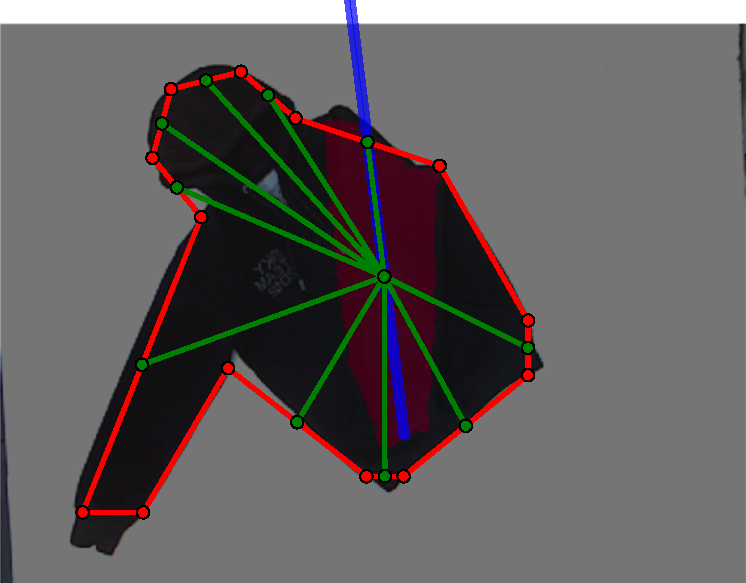
\includegraphics[width=\textwidth]
    	{figures/results/hoodie9-pnp.pdf}
	\end{subfigure} 
	~
	\begin{subfigure}[l]{\bigtablewidth}
	    \centering
    	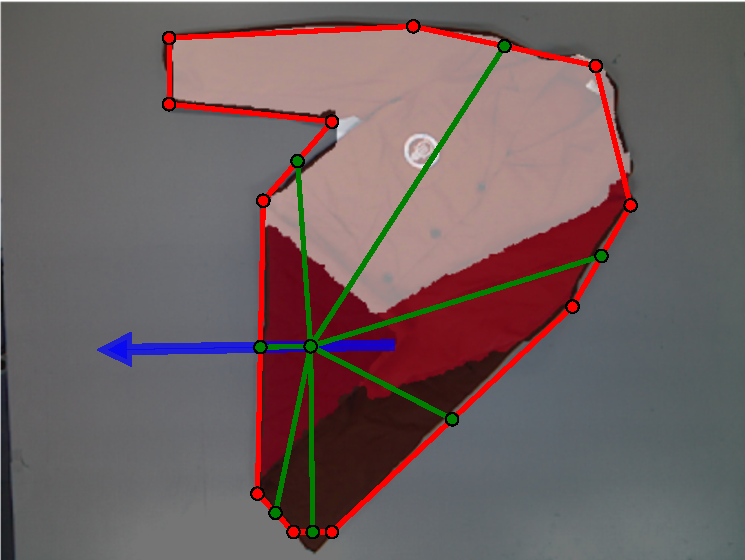
\includegraphics[width=\textwidth]
    	{figures/results/robe15-pnp.pdf}
	\end{subfigure}
	~
    \begin{subfigure}[r]{\bigtablewidth}
	    \centering
    	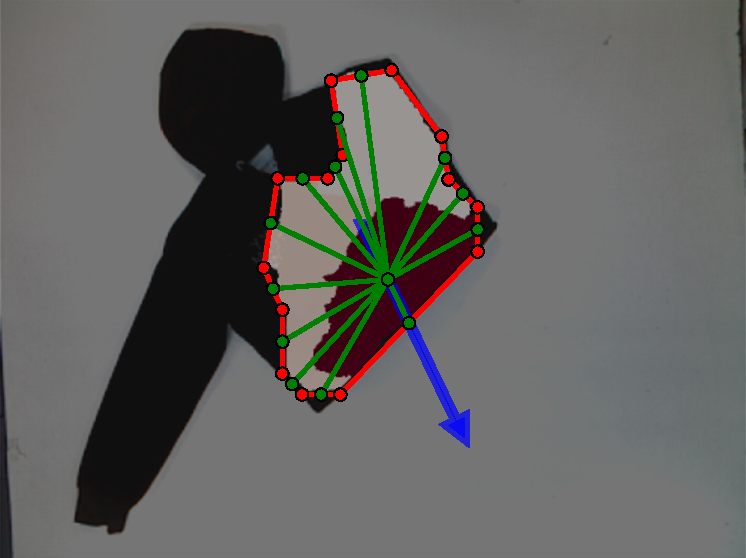
\includegraphics[width=\textwidth]
    	{figures/results/hoodie14-pnp.pdf}    	
	\end{subfigure}
	~
    \begin{subfigure}[l]{\bigtablewidth}
	    \centering
    	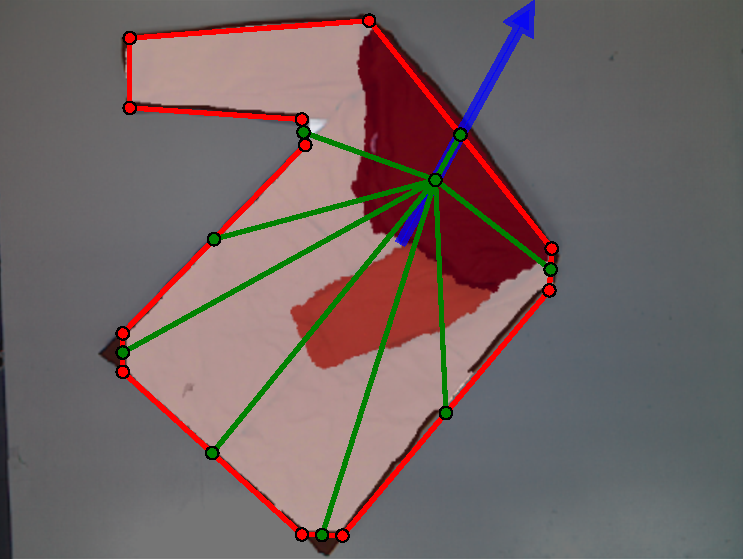
\includegraphics[width=\textwidth]
    	{figures/results/robe19-pnp.pdf}
	\end{subfigure}
	~
    \begin{subfigure}[r]{\bigtablewidth}
	    \centering
    	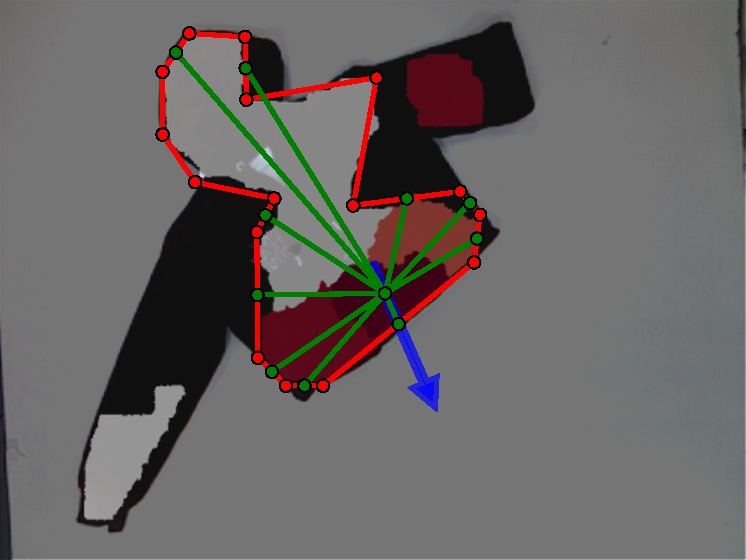
\includegraphics[width=\textwidth]
    	{figures/results/hoodie16-pnp.pdf}
	\end{subfigure} 
    \caption[Final output of the algorithm and the computed unfolding directions (Robe and Hoodie).]
    {Final output of the algorithm and the computed unfolding directions. Each column includes the output corresponding to 4 of the 20 database samples for each of the 6 garment categories considered. This figure includes the categories Robe and Hoodie.}
    \label{fig:results3}
\end{figure}


\comment{Lorem ipsum dolor sit amet, consectetur adipiscing elit. Donec a diam lectus. Sed sit amet ipsum mauris. Maecenas congue ligula ac quam viverra nec consectetur ante hendrerit. Donec et mollis dolor. Praesent et diam eget libero egestas mattis sit amet vitae augue. Nam tincidunt congue enim, ut porta lorem lacinia consectetur. Donec ut libero sed arcu vehicula ultricies a non tortor. Lorem ipsum dolor sit amet, consectetur adipiscing elit. Aenean ut gravida lorem. Ut turpis felis, pulvinar a semper sed, adipiscing id dolor. Pellentesque auctor nisi id magna consequat sagittis. Curabitur dapibus enim sit amet elit pharetra tincidunt feugiat nisl imperdiet. Ut convallis libero in urna ultrices accumsan. Donec sed odio eros. Donec viverra mi quis quam pulvinar at malesuada arcu rhoncus. Cum sociis natoque penatibus et magnis dis parturient montes, nascetur ridiculus mus. In rutrum accumsan ultricies. Mauris vitae nisi at sem facilisis semper ac in est.}

\section{Algorithm Validation}
\label{experiments:validation}

\comment{Bla, bla, bla.. validation.. bla, bla, bla}

\subsection{Experimental Setup}
\label{experiments:expermimental_setup}

The experimental setup consisted of several elements in a laboratory environment: a table, a depth sensor and a humanoid robot. The garment was placed on a white, flat surface, parallel to the floor. Over the garment, an ASUS Xtion PRO LIVE depth sensor was attached to a structure to capture data from a top view. The unfolding operation was performed by our full-body humanoid robot TEO \cite{martinez2012teo}. Figure \ref{fig:experimental_setup} depicts this setup.

\begin{figure}[t]
    \centering
    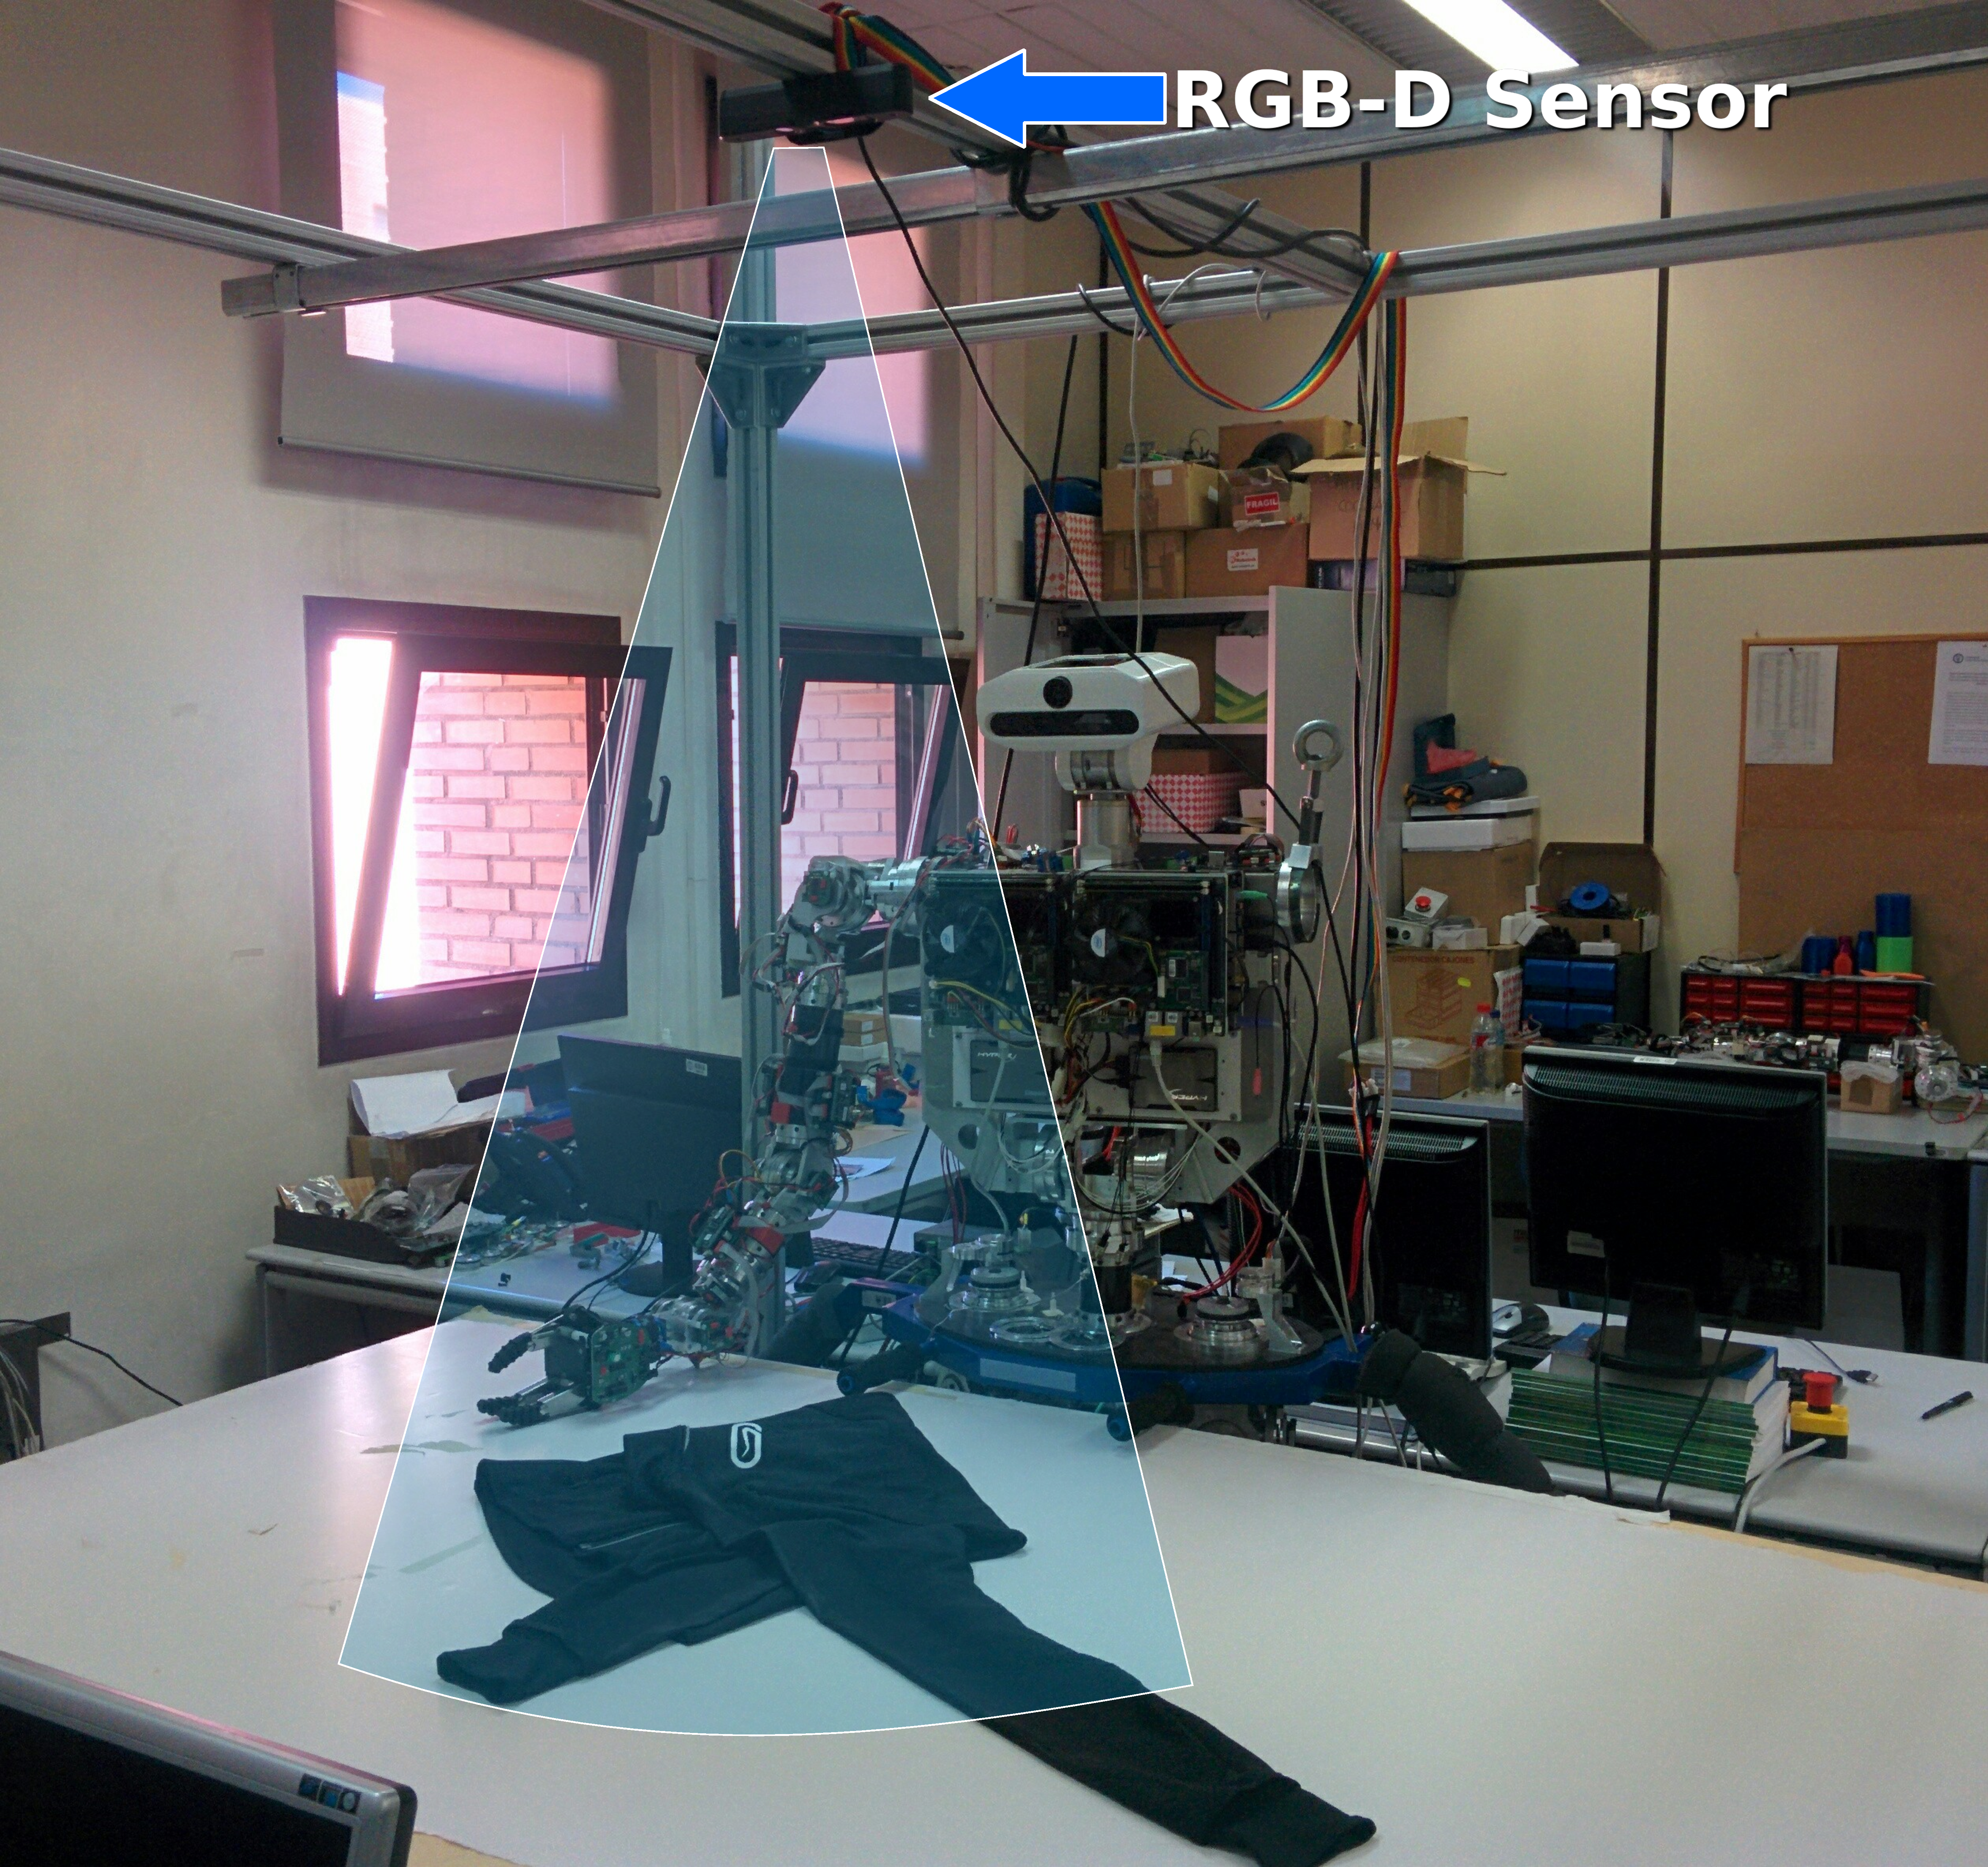
\includegraphics[width=0.8
    \textwidth]{figures/Experimental_setup.pdf}
    \caption[Experimental setup used to test the algorithm]
    {This figure shows the experimental setup used to test the algorithm. The garment rests over a flat white table, with the RGB-D sensor on top. Besides the table, the humanoid robot TEO waits for manipulation trajectories that indicate it how to perform the unfold action.}
    \label{fig:experimental_setup}
\end{figure}

The starting point for testing our algorithm is the data adquisition process. Data is obtained as a point cloud from a ASUS Xtion Pro Live sensor. Then, it is converted to a depth map image for its later analysis. 

This conversion is done by simply using the z component of each point as the depth value for each pixel of the depth image. If there were a known deviation from the surface (affecting perpendicularity), the depth image could be recovered from the point cloud using the instrinsic and extrinsic parameters of the sensor instead. As the sensor is placed on top of the garment, perpendicular to the surface on which the clothing article rests, both methods yield very similar results, as shown in figure \ref{fig:point_cloud_and_depth_image}.

\begin{figure}[htbp]
	\centering
    \begin{subfigure}[l]{0.9\textwidth}
	    \centering
    	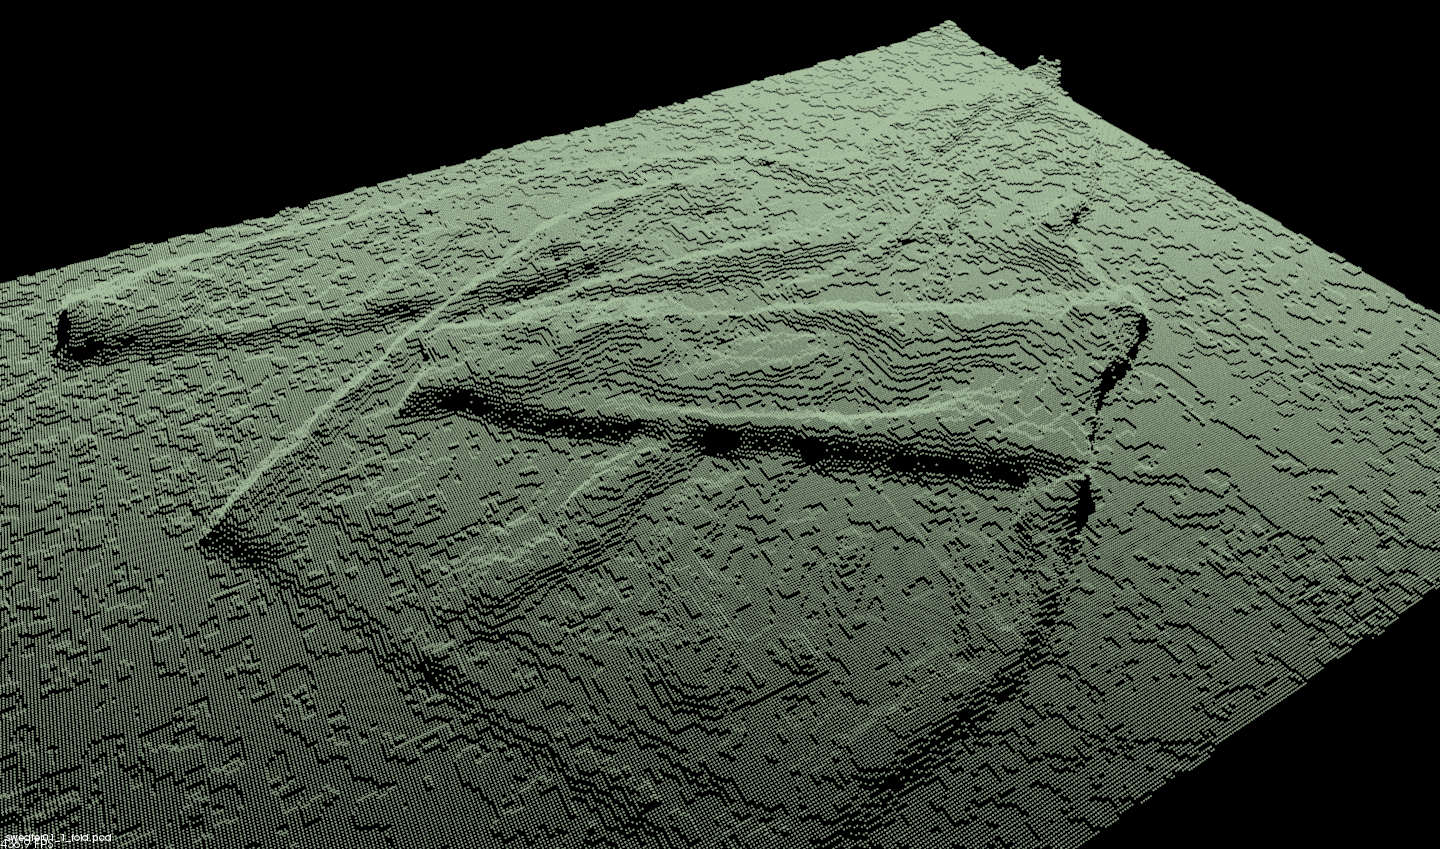
\includegraphics[width=\textwidth]
    	{figures/point-cloud-01.png}
    	\caption{3D Point cloud}
	\end{subfigure}
	~
    \begin{subfigure}[r]{0.9\textwidth}
	    \centering
    	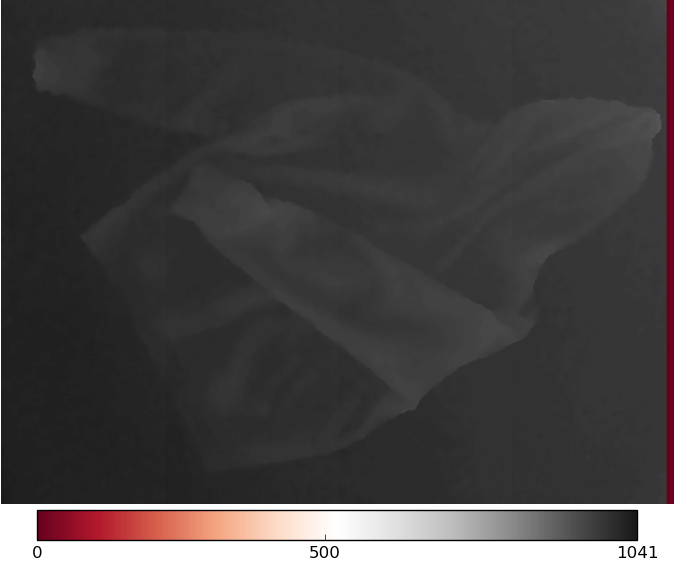
\includegraphics[width=\textwidth]
    	{figures/point-cloud-projection-2.png}
    	\caption{Depth Map}
	\end{subfigure}
    \caption[Comparison of the 3D point cloud with the Depth map obtained from its projection onto the table.]
    {Comparison of the 3D point cloud with the Depth map obtained from its projection onto the table. The colorbar beneath the second figure shows how depth from the camera (in mm) is mapped to the figure colors.}
    \label{fig:point_cloud_and_depth_image}
\end{figure}

The RGB values are also recorded for each depth image, obtaining an RGB-D image.

